\chapter{Umfrage}
\authortoc{\dario}{\chapterident}
Uns hat interessiert, wie der Lebensstil anderer Menschen aussieht und was für sie gesund Leben bedeutet. Aus diesem Grund haben wir eine Google Umfrage erstellt. Wir haben dann die Umfrage an alle Schüler unserer Schule und an Freunde und Bekannte in zwei Discord Servern versendet. Schlussendlich haben wir 110 Antworten erhalten.
\newline
Ich möchte darauf hinweisen, dass wir zuvor noch nie eine Umfrage erstellt haben und somit keine Erfahrungen damit haben. Wir haben zwei Fehler gemacht, welche wir erst nach versenden der Umfrage bemerkt haben. Wir haben einerseits vergessen, die Umfrage so einzustellen, dass eine Person die Umfrage nur einmal ausfüllen kann. Andererseits haben wir bei einer Multiple Choice Frage nicht alle Antwortmöglichkeiten abgedeckt.
\section{Auswertung}
\authortoc{\dario}{\sectionident}
\begin{figure}[H]
  \centering
  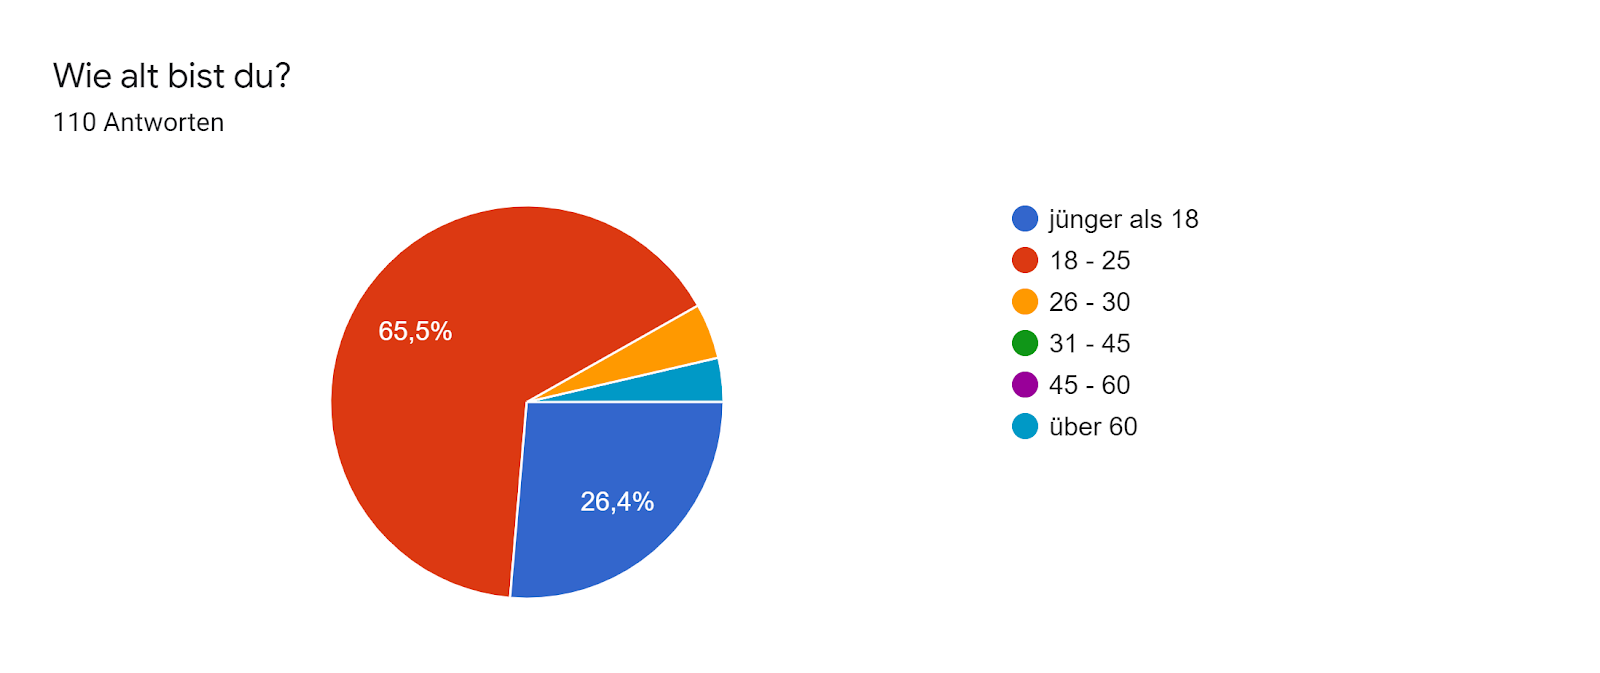
\includegraphics[width=0.7\linewidth]{./images/umfrage_a.png}
  \caption{Umfrage “Wie alt bist du?”}
  \label{fig:umfrage_a}
\end{figure}
\begin{figure}[H]
  \centering
  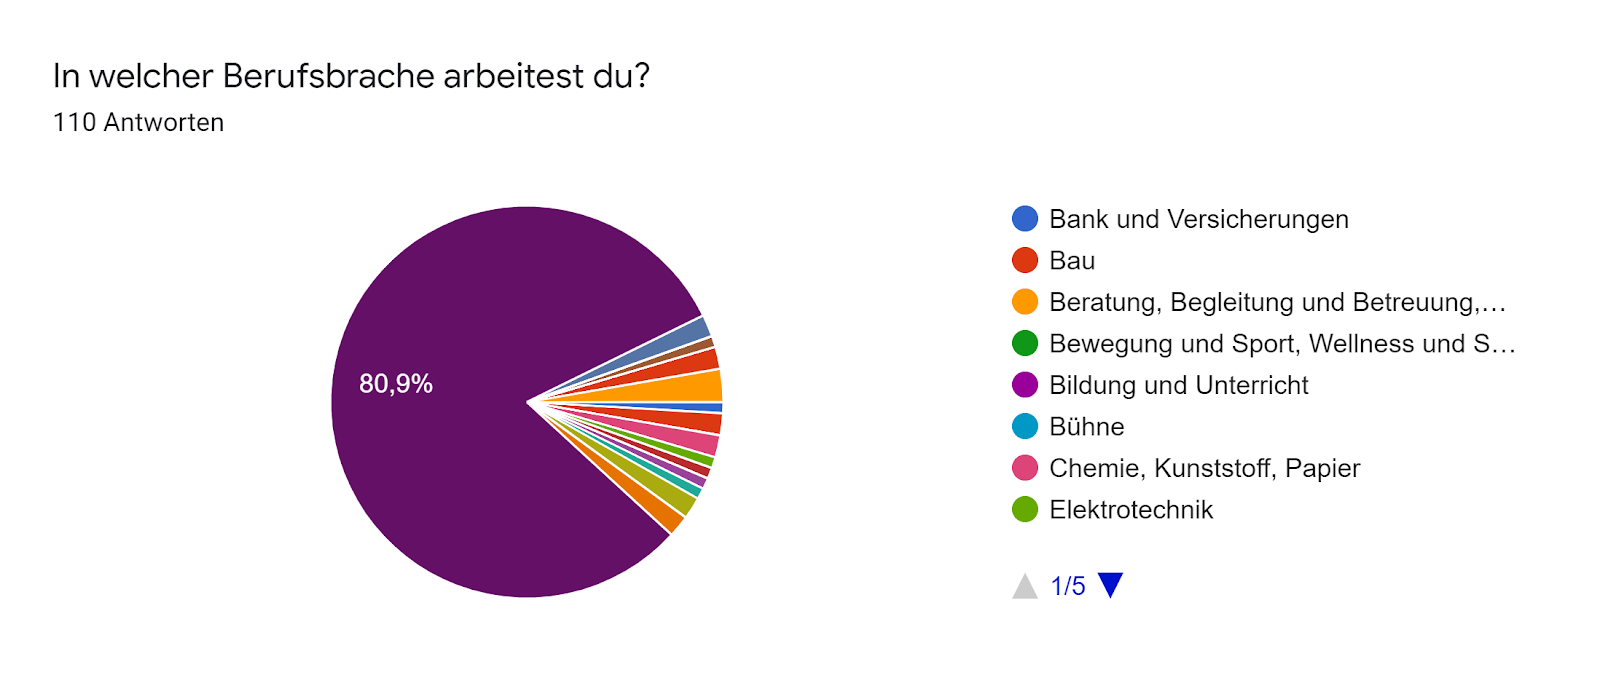
\includegraphics[width=0.7\linewidth]{./images/umfrage_b.png}
  \caption{Umfrage “In welcher Berufsbranche arbeitest du?}
  \label{fig:umfrage_b}
\end{figure}
Die ersten zwei Fragen haben wir gestellt um abschätzen zu können, was für Menschen unsere Umfrage ausgefüllt haben. Die meisten sind in unserem alter und sind in der “Informatik und Mediamatik (ICT)” Branche tätig. Dies haben wir bereits erwartet, da der grösste Teil, welche die Umfrage erhalten hat, Schüler unserer Schule sind.
\begin{figure}[H]
  \centering
  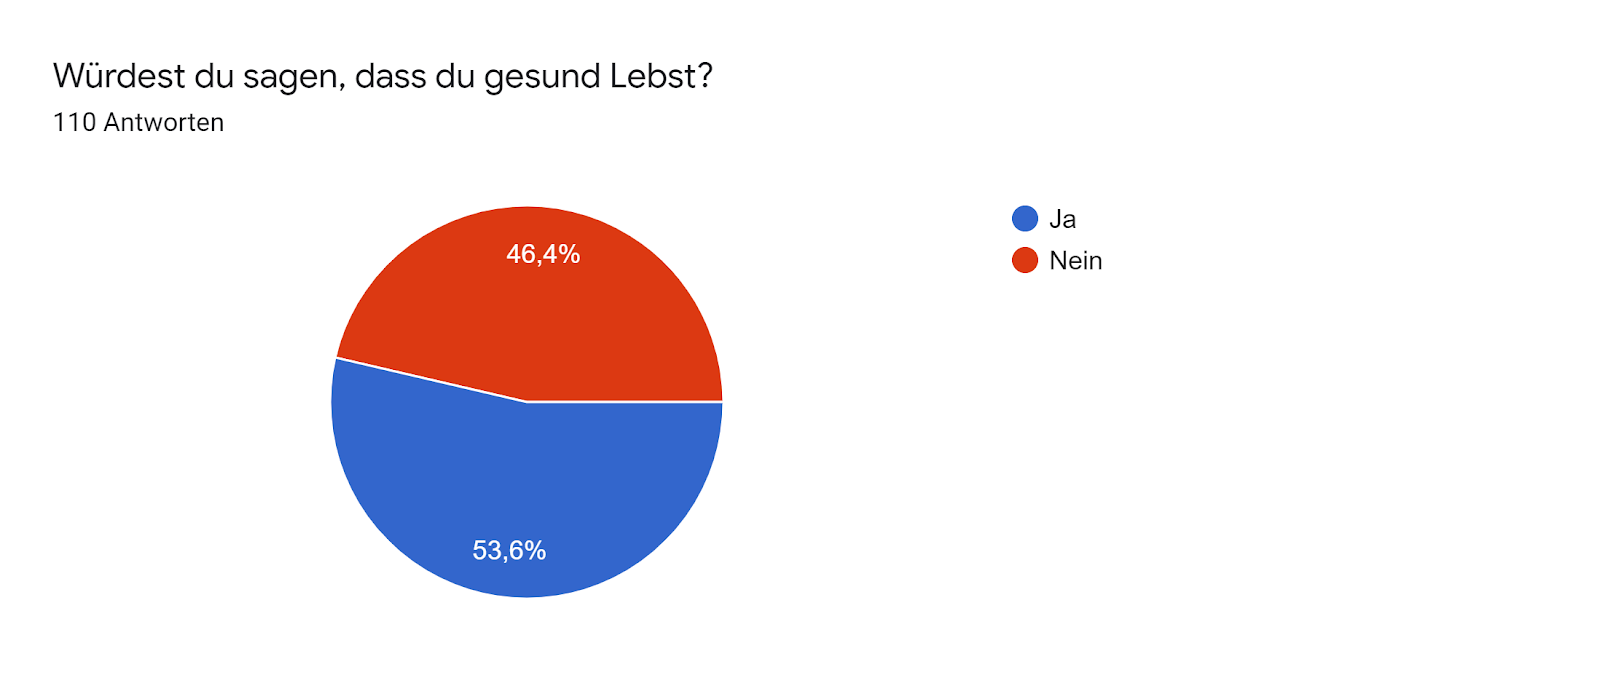
\includegraphics[width=0.7\linewidth]{./images/umfrage_c.png}
  \caption{Umfrage “Würdest du sagen, dass du gesund Lebst?”}
  \label{fig:umfrage_c}
\end{figure}
Die Mehrheit behauptet von sich, dass sie gesund leben. Dies hängt jedoch sehr stark davon ab, wie sie “gesund” definieren. Aber somit ist unsere annahme, dass mehr Menschen gesund leben als ungesund, korrekt. Jedoch habe wir eine klareres  “Ja” erwartet.
\begin{figure}[H]
  \centering
  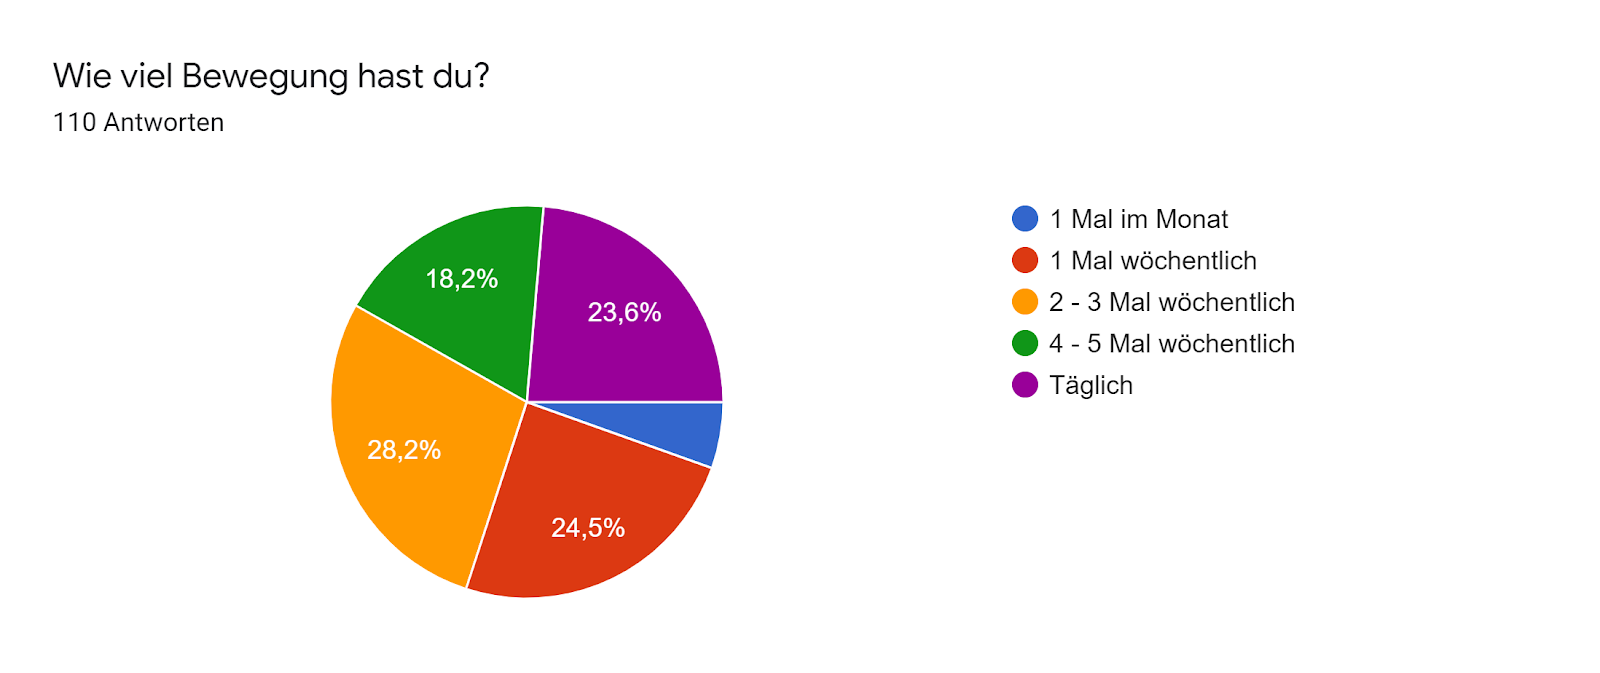
\includegraphics[width=0.7\linewidth]{./images/umfrage_d.png}
  \caption{Umfrage “Wie viel Bewegung hat du?”}
  \label{fig:umfrage_d}
\end{figure}
Die Antwort sind fast gleichmässig auf die Antwortmöglichkeiten verteilt. Bis auf die Antwortmöglichkeit “1 Mal im Monat”, welche nur sechs Personen selektiert haben. Auch diese Antworten, hängen stark davon ab, wie sie “bewegung” definiert haben. Die meisten, haben “2 - 3 Mal wöchentlich”, was wir auch in unserem Projekt versucht haben umzusetzen.
\begin{figure}[H]
  \centering
  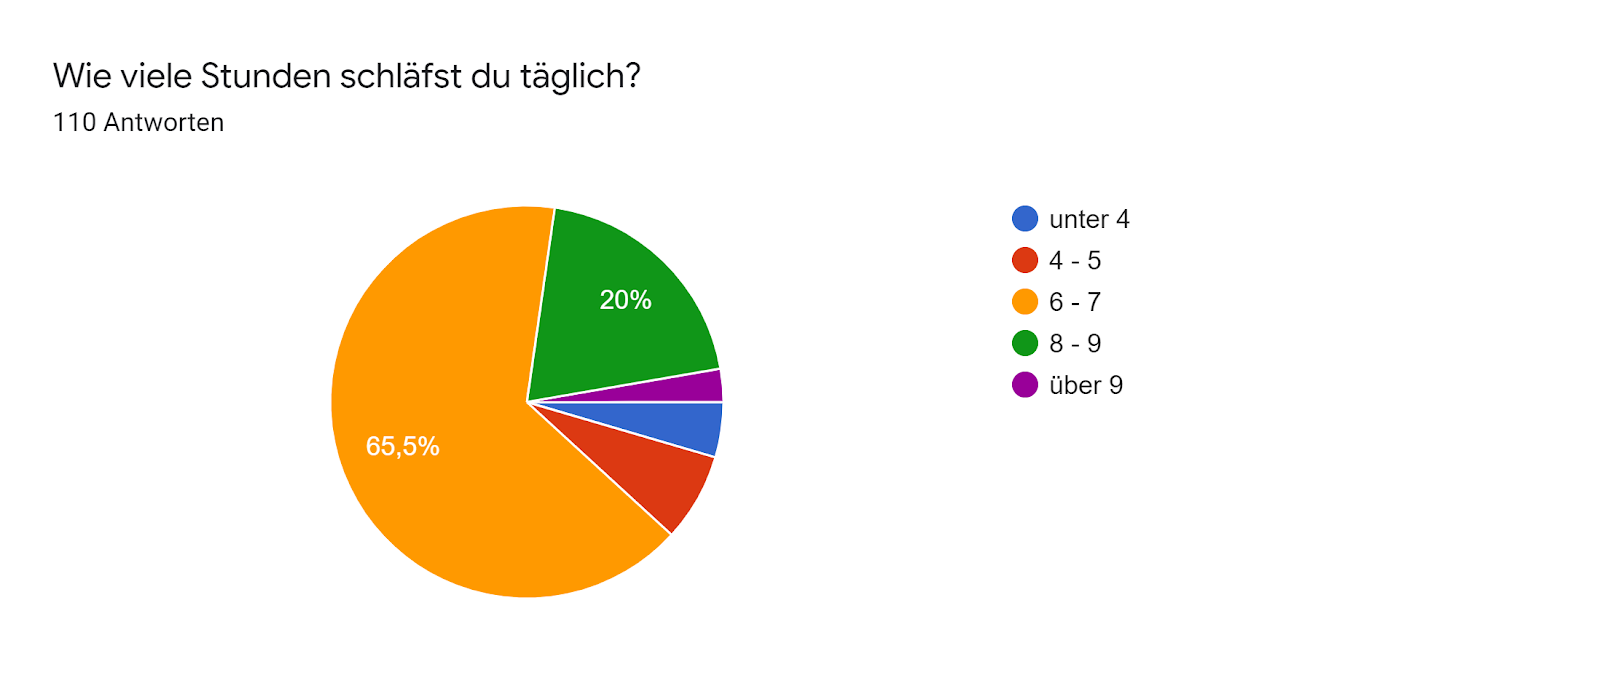
\includegraphics[width=0.7\linewidth]{./images/umfrage_e.png}
  \caption{Umfrage “Wie viel Stunden schläfst du täglich?”}
  \label{fig:umfrage_e}
\end{figure}
\begin{figure}[H]
  \centering
  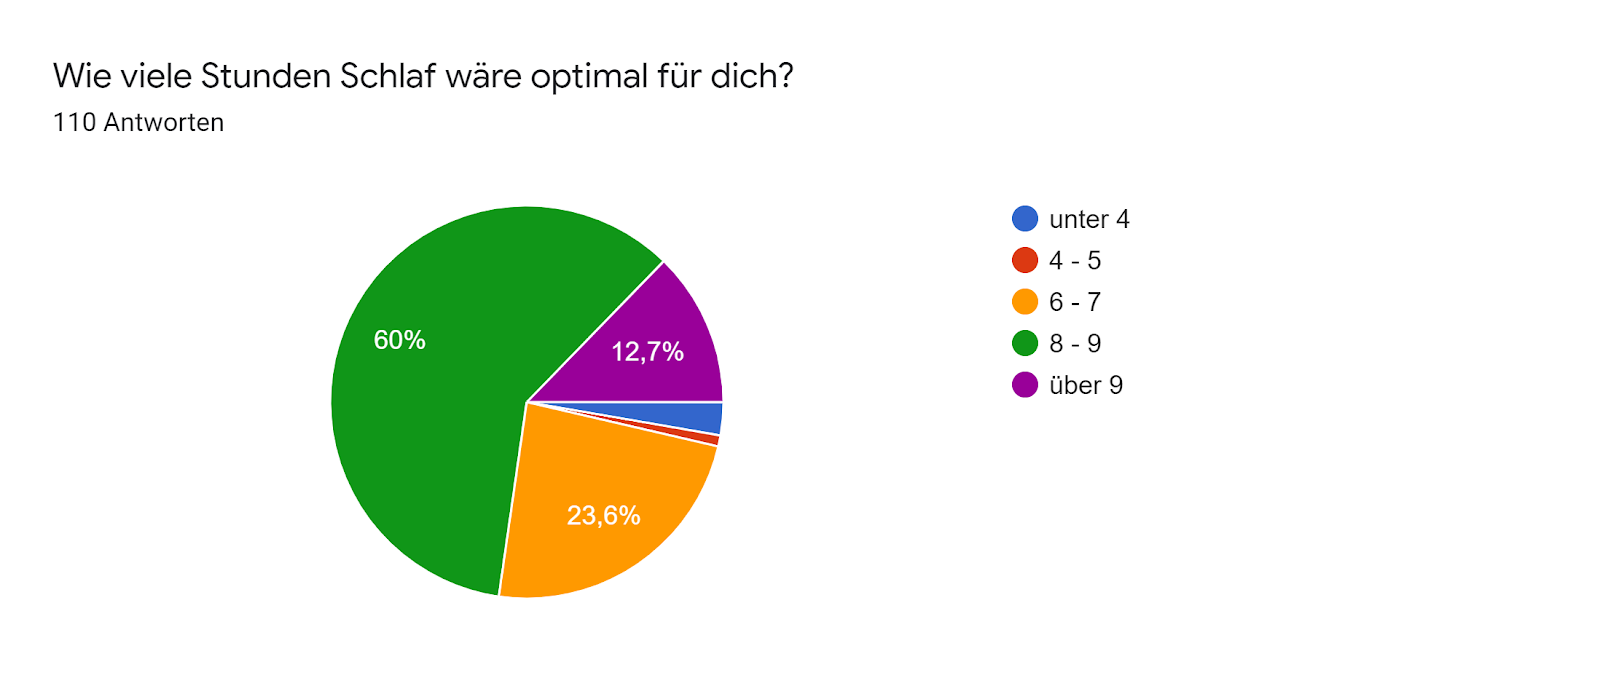
\includegraphics[width=0.7\linewidth]{./images/umfrage_f.png}
  \caption{Umfrage “Wie viel Stunden Schlaf wäre optimal für dich?”}
  \label{fig:umfrage_f}
\end{figure}
Hier haben wir den Fehler gemacht, nicht alle Antwortmöglichkeiten zu geben.
\newline
Die Mehrheit schläft zwischen 6 und 7 Stunden pro nacht und für die Mehrheit wäre 8 -9 Stunden Optimal. Wenn man nun die zwei Grafiken vergleicht sieht man, dass die meisten zu wenig schlafen.
\begin{figure}[H]
  \centering
  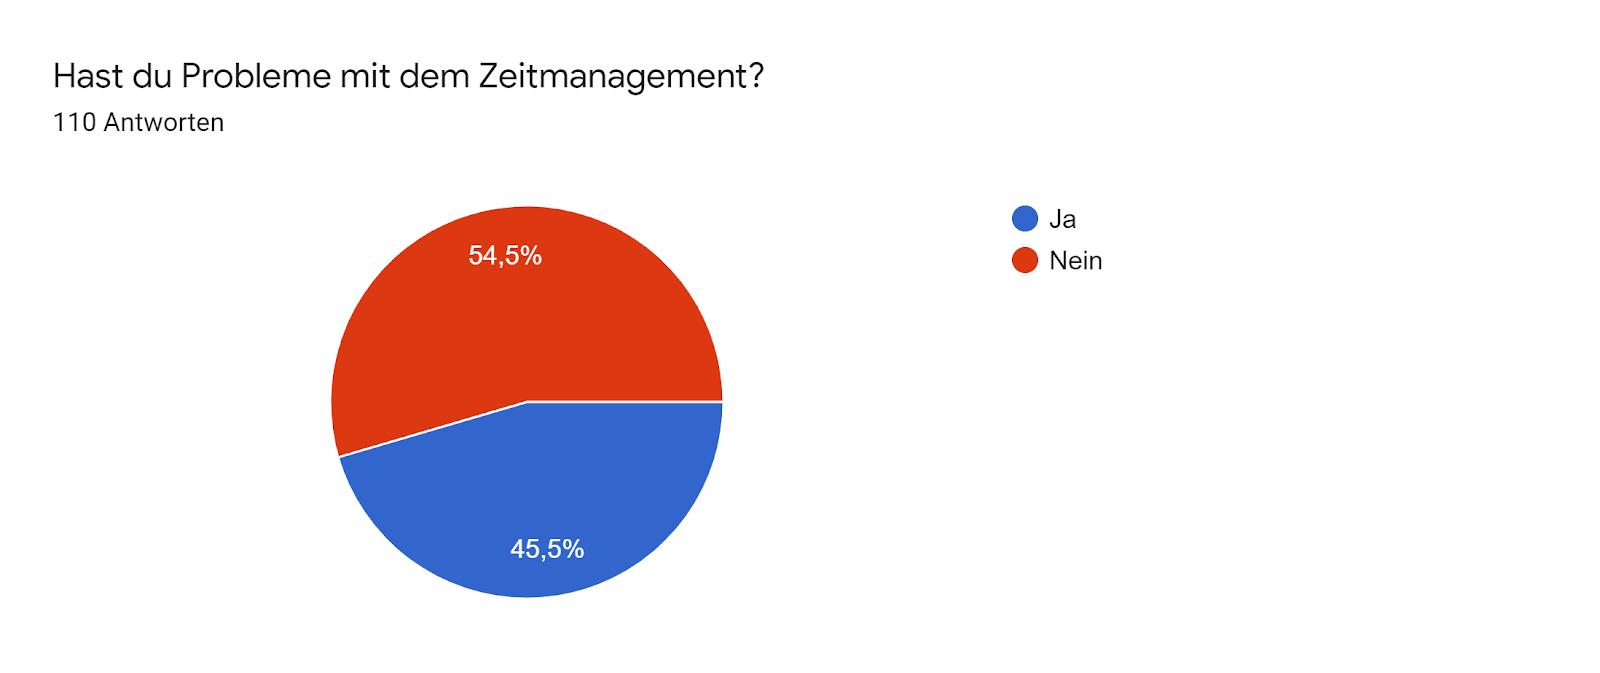
\includegraphics[width=0.7\linewidth]{./images/umfrage_g.png}
  \caption{Umfrage “Hast du Probleme mit dem Zeitmanagement?”}
  \label{fig:umfrage_g}
\end{figure}
Die Mehrheit hat keine Probleme mit dem Zeitmanagement. Die Verteilung, der Antworten ist sehr ähnlich mit der Verteilung der Antworten der Frage “Würdest du sagen, dass du gesund Lebst?”.
\subsection{Beschreibe in einem kurzen Satz, was für die gesund bedeutet}
\authortoc{\dario}{\subsectionident}
Da ich nicht alle 110 Antworten hier festhalten kann, habe ich versucht, so gut es ging, diese zusammenzufassen.
\newline
Gesund bedeutet keine Psychische und Physische Einschränkungen zu haben. Dazu soll man ausgewogen und stressfrei leben, auf die Ernährung achten und genug Sport treiben. Wichtig ist, dass man glücklich ist.